O HSM é composto de duas estruturas com saliências, o rotor e o estator, seu circuito magnético é excitado pela combinação de espiras e magnetismo permanente, imã. As espiras são montadas nos polos do estator e o imã no rotor. Tipicamento o motor de passo híbrido tem oito polos no estator e em cada polo tem entre dois a seis dentes, ou também chamado \emph{teeth}, do inglês. Ele tem ainda comumente um pequeno largura de passo, tipicamente 1,8º. Como mostrado na Figura \ref{fig:estrutura_HSM}. \cite{SteppingBook}

\begin{figure}[!h]
	\centering
	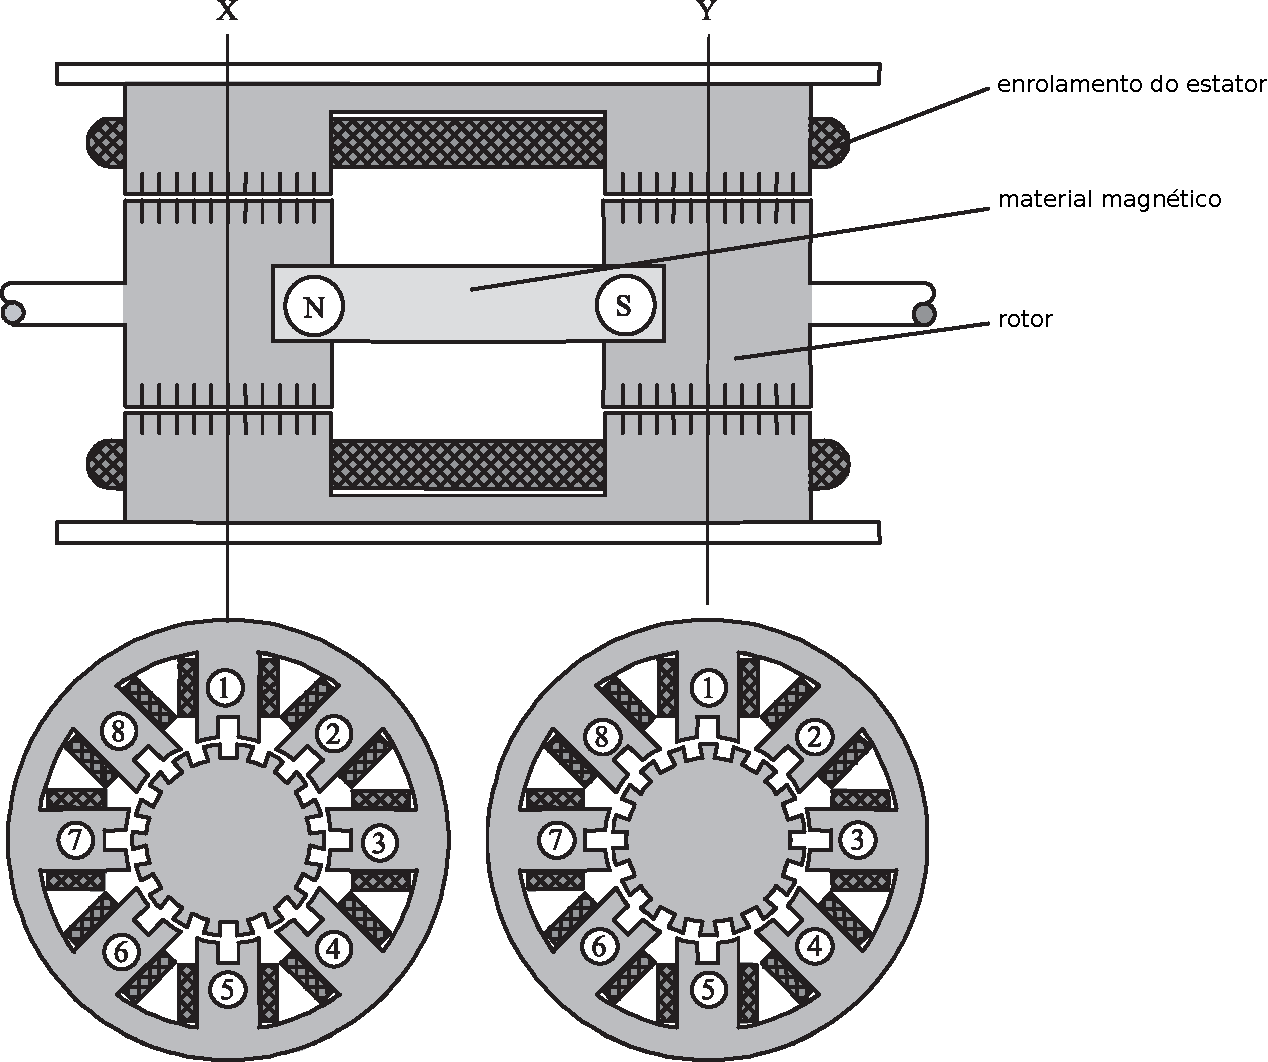
\includegraphics[width = \columnwidth]{Images/estrutura_HSM.pdf}
	\caption{Visão de lado, frente e costas do HSM. \cite{SteppingBook}}
	\label{fig:estrutura_HSM}
\end{figure}

O rotor é construído de tal forma que os dentes do polo sul fiquem alinhados entre dois dentes do polo norte, mais claramente percebível na Figura \ref{fig:HSM_dentes}.

\begin{figure}[!h]
	\centering
	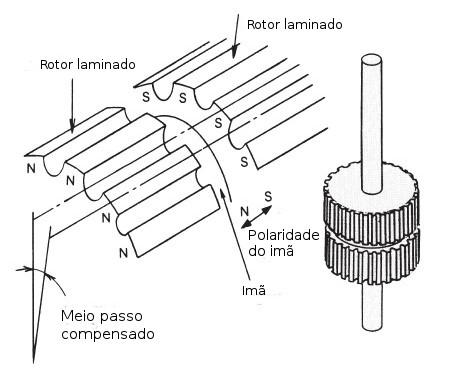
\includegraphics[width = \columnwidth]{Images/VR_ROTOR.jpg}
	\caption{Detalhe de construção do rotor do HSM. \cite{angulo_rotor}}
	\label{fig:HSM_dentes}
\end{figure}

As principais partes constituintes de um HSM comercial é mostrado na Figura \ref{fig:partes_SM}.

\begin{figure}[!h]
	\centering
	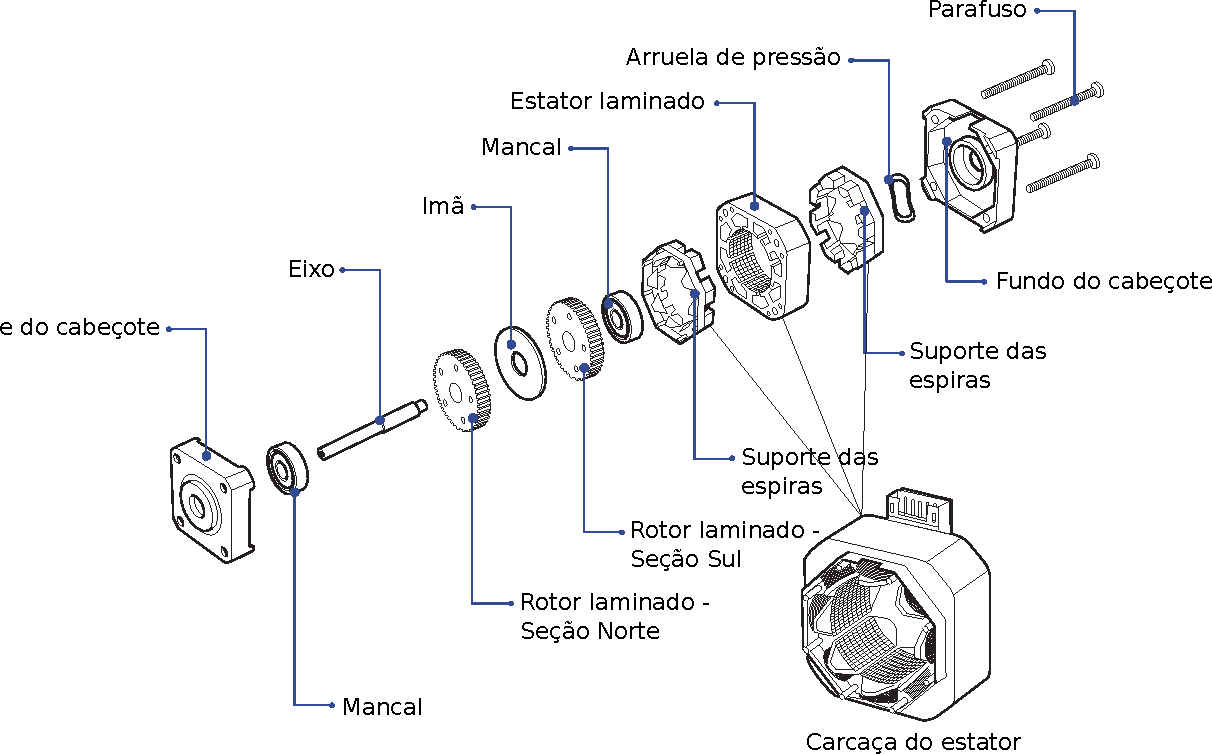
\includegraphics[width = \columnwidth]{Images/partes_HSM.pdf}
	\caption{Partes constituintes de um HSM comercial. \cite{MoonsHSM}}
	\label{fig:partes_SM}
\end{figure}
